\newpage
\section*{CHAPTER 5. RESULTS}
\addcontentsline{toc}{section}{\numberline{}CHAPTER 5. RESULTS}
\setcounter{section}{5}
\setcounter{subsection}{0}
\setcounter{subsubsection}{0}
\setcounter{paragraph}{0}
\setcounter{figure}{0}
\setcounter{table}{0}






\subsection{Quantization Results and Evaluation}

This section presents the experimental evaluation of the mixed-precision quantization applied to the HiFiC-Hi model. The objective is to assess the impact of transitioning from full-precision FP32 computation to a mixed-precision FP16 implementation on compression efficiency and reconstructed image quality.

Experiments were conducted on a representative test image with a resolution of $256 \times 256$. Two configurations were compared under identical conditions: the baseline FP32 model and the quantized mixed-precision FP16 model, where internal computations operate in FP16 while input and output interfaces remain in FP32.

Table~\ref{tab:quant_results} summarizes the quantitative compression metrics obtained from both models.

\begin{table}[H]
\centering
\caption{Comparison between FP32 and FP16 mixed-precision HiFiC models}
\label{tab:quant_results}
\begin{tabular}{|l|c|c|c|}
\hline
\textbf{Metric} & \textbf{FP32} & \textbf{FP16 Mixed} & \textbf{Delta} \\
\hline
Original Size (bytes) & 25,879 & 25,879 & 0 \\
Bitstream Size (bytes) & 6,522 & 6,517 & -5 \\
Output Image Size (bytes) & 97,596 & 97,496 & -100 \\
Compression Ratio & 3.97$\times$ & 3.97$\times$ & 0.00 \\
Space Saving (\%) & 74.80 & 74.82 & +0.02 \\
Bits Per Pixel (bpp) & 0.7961 & 0.7955 & -0.0006 \\
PSNR (dB) & 19.08 & 19.05 & -0.03 \\
SSIM & 0.8315 & 0.8314 & -0.0001 \\
MSE  &  804.315755 & 808.560496 & 4.244 \\
\hline
\end{tabular}
\end{table}

The results indicate that the compression performance of the HiFiC model is preserved after quantization. The bitstream size is slightly reduced, while the compression ratio and space-saving metrics remain unchanged. This suggests that the probability distribution of the latent representation is not significantly affected by FP16 rounding errors, allowing the entropy coding process to operate efficiently.

From a perceptual quality perspective, the degradation introduced by mixed-precision computation is negligible. The observed PSNR reduction of 0.03~dB is well below the threshold of perceptual visibility, and the SSIM metric remains nearly identical between the two configurations. These results confirm that structural features and texture details are effectively preserved under FP16 computation.

Figure~\ref{fig:quant_visual} provides a visual comparison between the reconstructed images produced by the FP32 and FP16 models.

\begin{figure}[H]
    \centering
    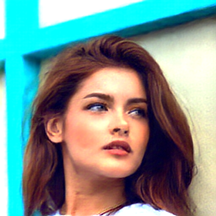
\includegraphics[width=0.45\linewidth]{Images/originial.png}
    \hfill
    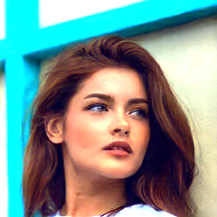
\includegraphics[width=0.45\linewidth]{Images/quantized picture.png}
    \caption{Visual comparison of reconstructed images: FP32 model (left) and FP16 mixed-precision model (right)}
    \label{fig:quant_visual}
\end{figure}

No visible artifacts or structural distortions are observed in the quantized output. Overall, the experimental results demonstrate that the proposed mixed-precision quantization strategy achieves a favorable balance between numerical efficiency and output fidelity, validating its suitability for FPGA deployment of the HiFiC image compression model.

\subsection{Verification and Evaluation Overview}

This chapter presents the quantization, verification, and implementation results of the proposed HiFiC GAN accelerator. The remaining evaluation focuses on functional correctness, FPGA resource utilization, waveform-based simulation, comparison with the Python reference model, and board-level execution on the ZCU104 platform.

After completing the coding and simulation process, we synthesized the source code to evaluate the performance and resource utilization of the circuit. 

\subsubsection{Generative Adversarial Network}
\paragraph{Results after Synthesis}

We obtained results after synthesizing the GAN circuit, including: DSP, FF, LUT, and DRAM Utilization Parameters in the GAN Block:





\begin{table}[htbp]
\centering
\caption{Utilization Report}
\label{tab:utilization_report}
\resizebox{\textwidth}{!}{%
\begin{tabular}{lcccccccccccc}
\toprule
\textbf{Name} & \textbf{\begin{tabular}[c]{@{}c@{}}CLB LUTs\\ (230400)\end{tabular}} & \textbf{\begin{tabular}[c]{@{}c@{}}CLB Regs\\ (460800)\end{tabular}} & \textbf{\begin{tabular}[c]{@{}c@{}}CARRY8\\ (28800)\end{tabular}} & \textbf{\begin{tabular}[c]{@{}c@{}}F7 Mux\\ (115200)\end{tabular}} & \textbf{\begin{tabular}[c]{@{}c@{}}F8 Mux\\ (57600)\end{tabular}} & \textbf{\begin{tabular}[c]{@{}c@{}}CLB\\ (28800)\end{tabular}} & \textbf{\begin{tabular}[c]{@{}c@{}}LUT Logic\\ (230400)\end{tabular}} & \textbf{\begin{tabular}[c]{@{}c@{}}LUT Mem\\ (101760)\end{tabular}} & \textbf{\begin{tabular}[c]{@{}c@{}}BRAM Tile\\ (312)\end{tabular}} & \textbf{\begin{tabular}[c]{@{}c@{}}URAM\\ (96)\end{tabular}} & \textbf{\begin{tabular}[c]{@{}c@{}}DSPs\\ (1728)\end{tabular}} & \textbf{\begin{tabular}[c]{@{}c@{}}BUFGCE\\ (208)\end{tabular}} \\ \midrule
design\_1\_wrapper & 57291 & 73774 & 1579 & 1695 & 724 & 12198 & 52406 & 4885 & 105 & 76 & 48 & 2 \\
\hspace{0.5cm} dbg\_hub & 447 & 753 & 7 & 0 & 0 & 135 & 427 & 20 & 0 & 0 & 0 & 1 \\
\hspace{0.5cm} design\_1\_i & 56844 & 73021 & 1572 & 1695 & 724 & 12066 & 51979 & 4865 & 105 & 76 & 48 & 1 \\ \bottomrule
\end{tabular}%
}
\end{table}
We continued evaluating and documenting the resource usage in the GAN block, ensuring optimal resource utilization. We measured and verified the processing time parameters of the GAN circuit.




\paragraph{Main Blocks of the GAN Circuit}
We listed and described the main blocks in the GAN circuit, providing a clear understanding of the structure and interactions between components.
\begin{figure}[H]
    \centering
    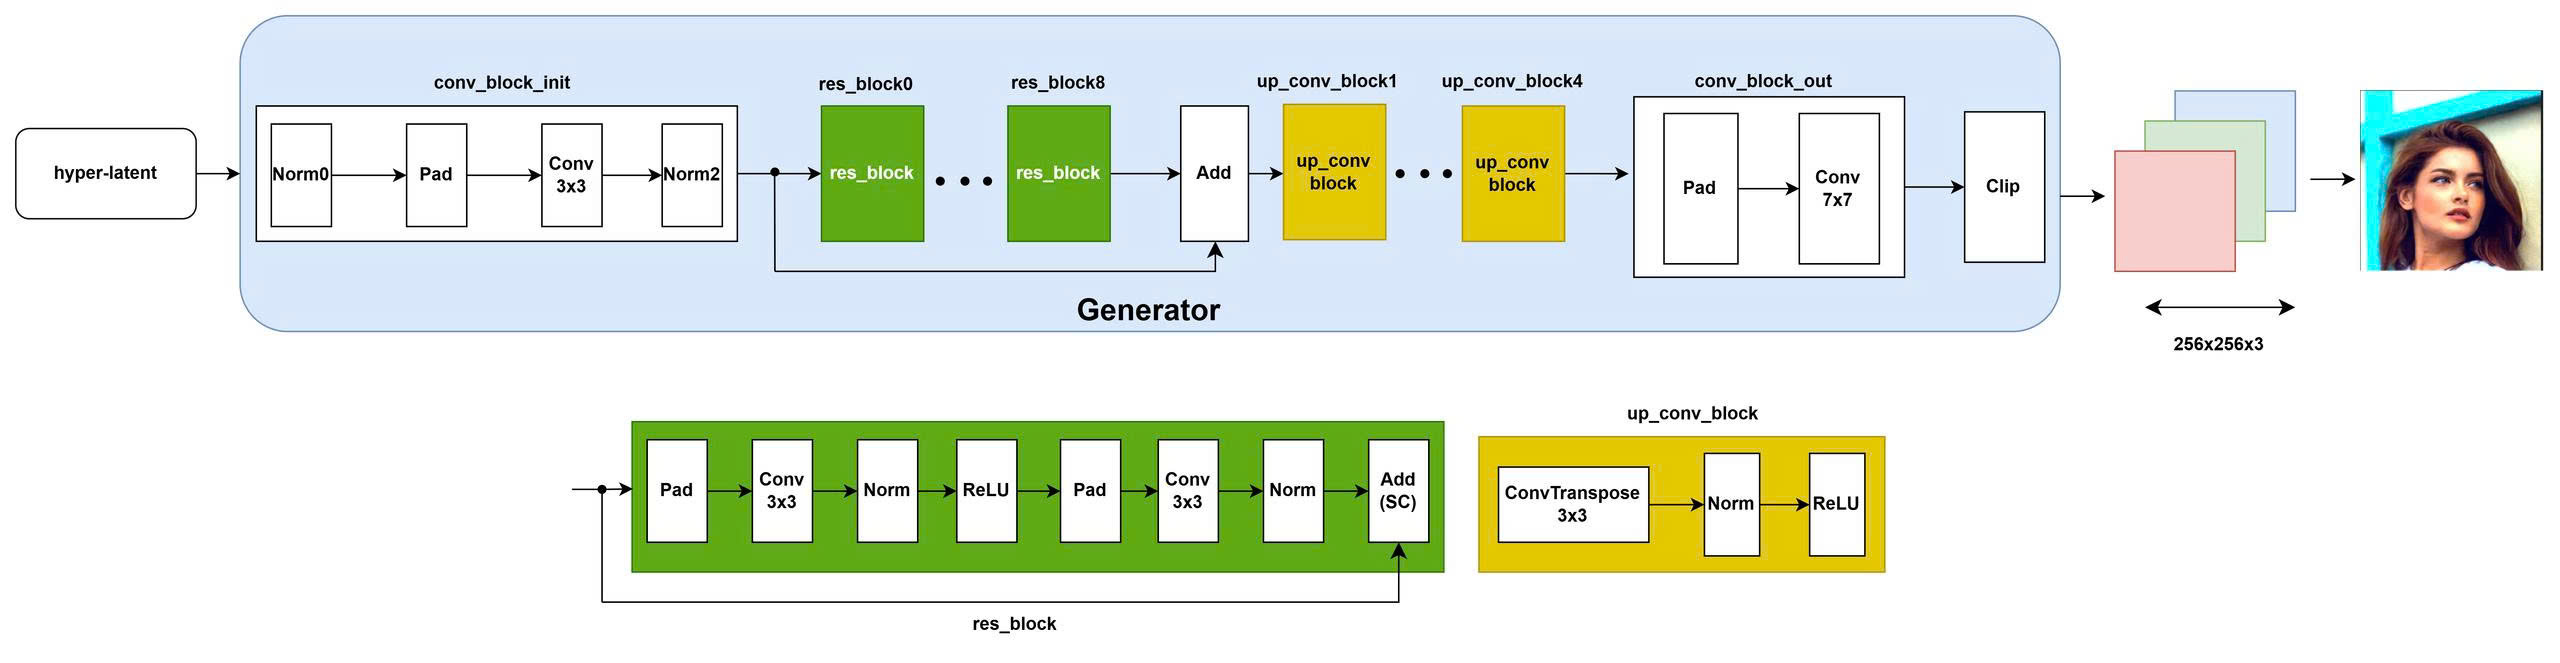
\includegraphics[width=0.8\linewidth]{Images/GAN_Block.jpg}
    \caption{Main GAN block}
    \label{GANblock}
\end{figure}

This information offers a detailed and comprehensive view of the performance, resource utilization, and structure of GAN after the synthesis and simulation process. This data serves as a foundation for further optimization and adjustments to the circuit if necessary.

\paragraph{GAN Results}
We created waveforms to visualize the correspondence between the input and output data during the generating process. The following aspects were observed and analyzed. We compared the input data with the corresponding output data, ensuring that the decoding process produced the expected results.

\begin{figure}[H]
    \centering
    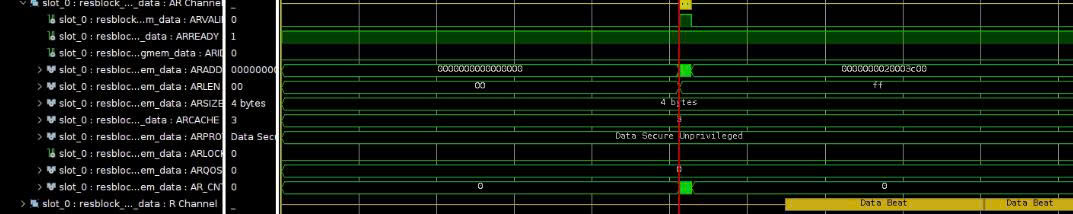
\includegraphics[width=1\linewidth]{Images/waveform.jpg}
    \caption{Input Data}
    \label{fig:gan_waveform}
\end{figure}
\begin{figure}[H]
    \centering
    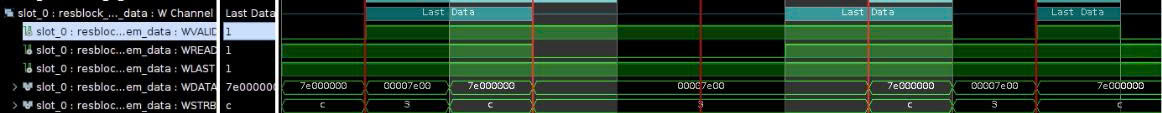
\includegraphics[width=1\linewidth]{Images/wave_w.jpg}
    \caption{Output Data}
    \label{fig:gan_weight_waveform}
\end{figure}



\subsection{Comparison with Python Reference}
Next, the HLS simulation results are compared with the Python reference model using PSNR as the key reconstruction-quality metric for the quantized hardware-oriented implementation.

\begin{figure}[H]
    \centering
    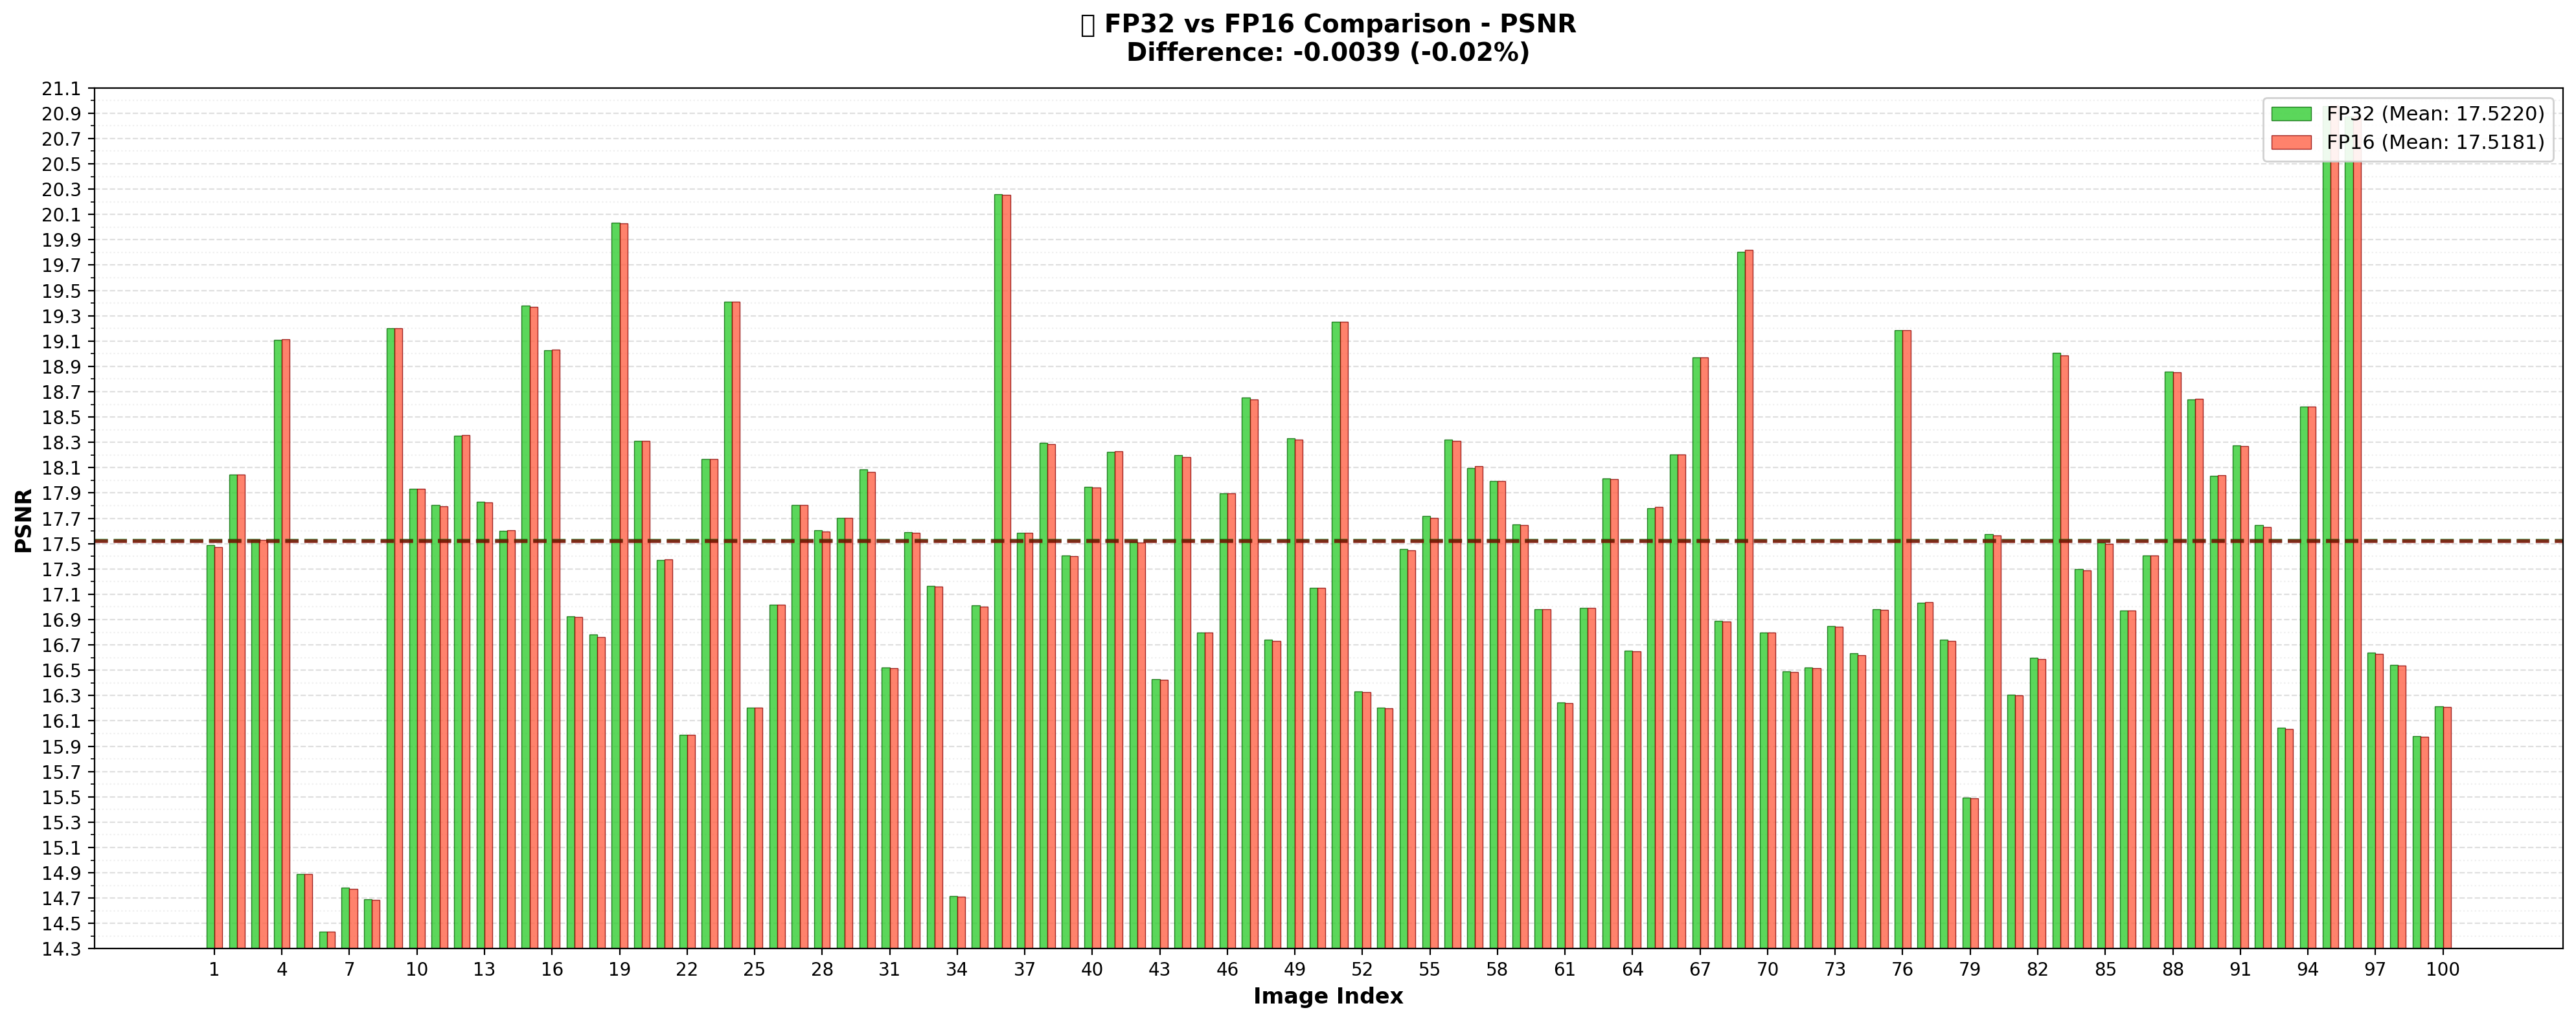
\includegraphics[width=1\linewidth]{Images/comparison_psnr_sidebyside.png}
    \caption{Comparison between the Python reference model and the quantized HLS simulation model}
    \label{psnr}
\end{figure}


Figure~\ref{psnr} depicts the PSNR results of 100 images evaluated using the Python reference model and the quantized HLS simulation model. The results demonstrate the similarity between the software reference and the hardware-oriented implementation. The accelerator design is tested on the ZCU104 platform as part of the complete FPGA deployment flow.

\subsection{Implementation on ZCU104}
After creating the complete SoC block design, the system was synthesized, implemented, and exported as a bitstream for the ZCU104 platform using Vivado. A Vitis application was then developed to control the accelerator and measure the end-to-end latency. The FPGA implementation achieves an approximately five-times speedup compared with the software-only measurement at an operating frequency of 300~MHz. 


\begin{figure}[H]
    \centering
    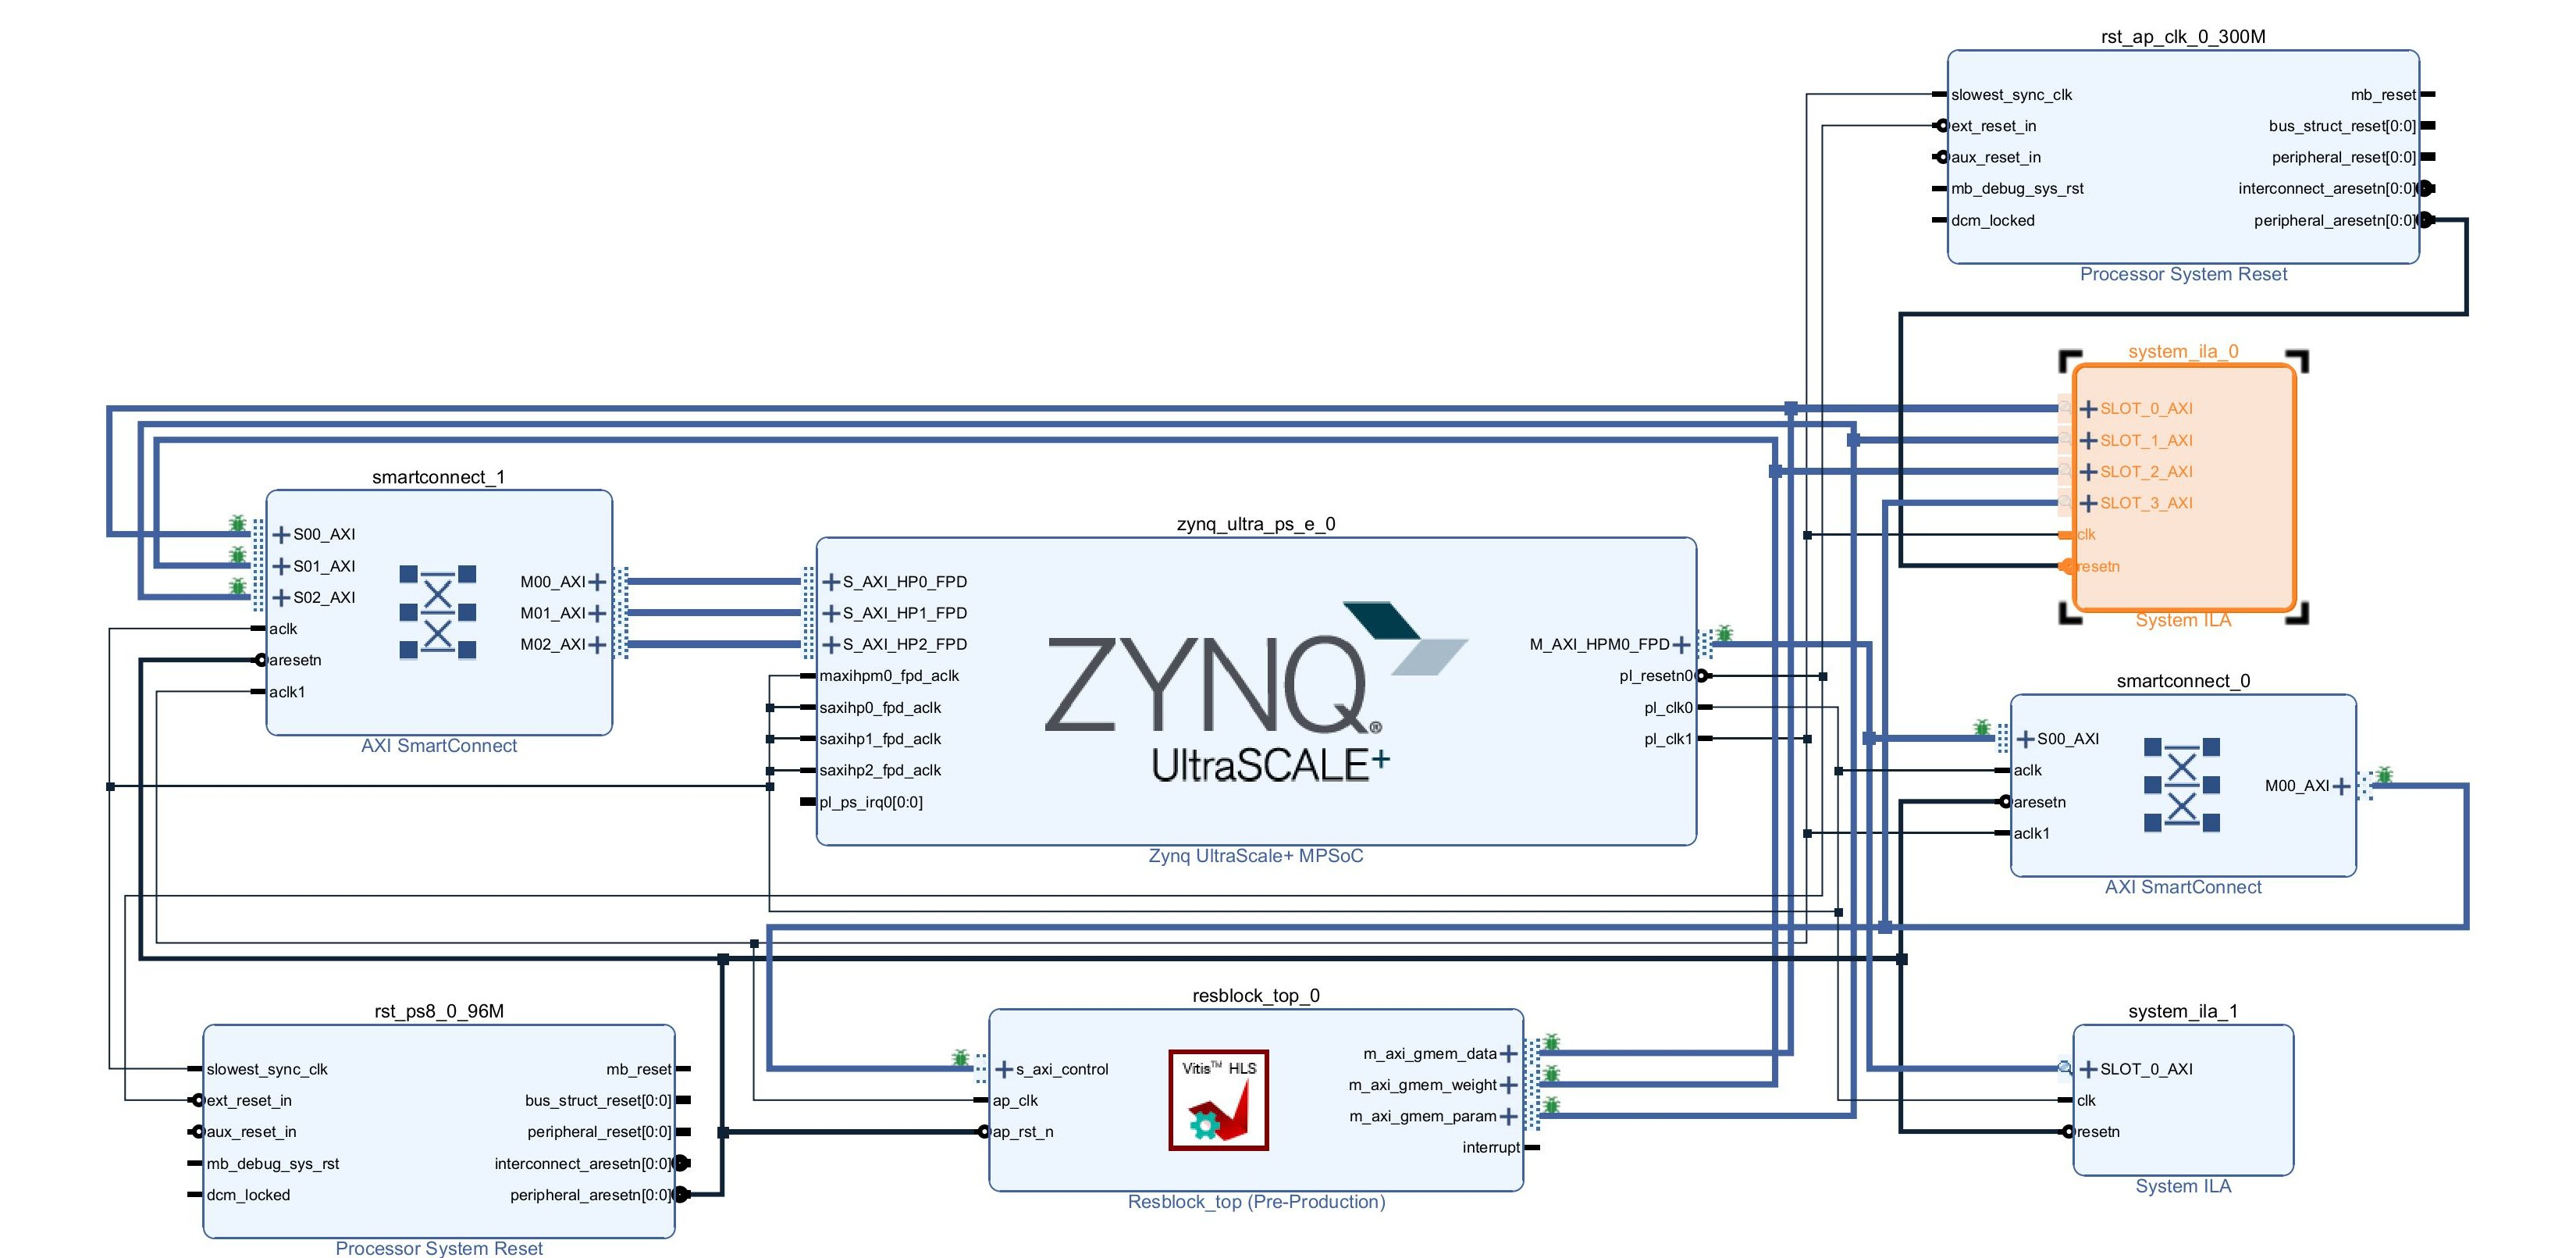
\includegraphics[width=1\linewidth]{Images/block_design.jpg}
    \caption{Block design for FPGA}
    \label{Block design for FPGA}
\end{figure}